% !TeX root = main.tex

\hypertarget{monotonicity-and-concavity}{%
\section{Monotonicity and Concavity}\label{monotonicity-and-concavity}}

\hypertarget{monotonicity-test}{%
\subsection{Monotonicity Test}\label{monotonicity-test}}

\begin{proposition}

\textbf{(Increasing/Decreasing Test)} Let \(f\) be a function
differentiable on an interval \(I\).

\begin{enumerate}[sepno]
\item
  If \(f'(x)>0\) on an interval \(I\), then f is increasing on that
  interval \(I\).
\item
  If \(f'(x)<0\) on an interval \(I\), then f is decreasing on that
  interval \(I\).
\end{enumerate}

\end{proposition}

\begin{example}

Show that \(f(x)=x^2-2x\) is decreasing on \((-\infty, 1)\) and
increasing on \((1,\infty)\).

\end{example}
\vspace*{6\baselineskip}

\begin{example}

Find intervals where \(f(x)=x-2\cos x\) is increasing or decreasing.

\end{example}
\vspace*{6\baselineskip}

\begin{proposition}

\textbf{(First Derivative Test for a Local Extremum)} Let \(f\) be a
function continuous on \((a, b)\) and differentiable on
\((a, b)\setminus\{c\}\).

\begin{enumerate}[sepno]
\item
  If \(f'(x)\) chance from positive to negative when \(x\) moves to the
  right passing \(c\), then \(f\) has a local maximum at \(c\).
\item
  If \(f'(x)\) chance from negative to positive when \(x\) moves to the
  right passing \(c\), then \(f\) has a local minimum at \(c\).
\item
  If \(f'(x)\) has the same sign on both sides of \(c\), then \(f\) does
  not have a local extremum at \(c\).
\end{enumerate}

\begin{fullwidth}
  \centering
  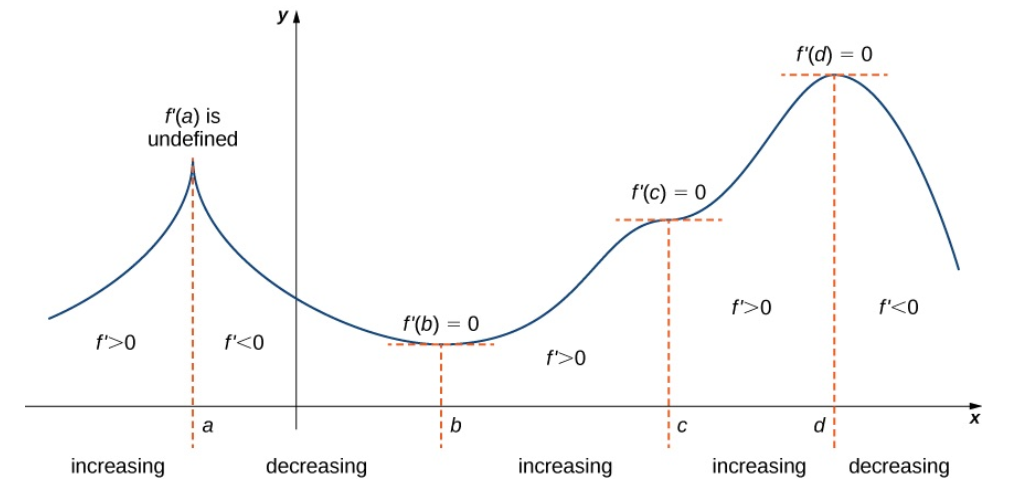
\includegraphics[width=0.8\linewidth]{img/image-20200413134520221.png}
\end{fullwidth}

\end{proposition}

\begin{example}

Use the first derivative test to find the location of all local extrema
for \(f(x)=x^3 - 3x^2 - 9x - 1\).

\end{example}
\vspace*{6\baselineskip}

\begin{example}

Use the first derivative test to find the location of all local extrema
for \(f(x)=5x^{1/3} - x^{5/3}\).

\end{example}
\vspace*{6\baselineskip}

\hypertarget{concavity-test}{%
\subsection{Concavity Test}\label{concavity-test}}

\begin{definition}

If the graph of \(f\) lies above all of its tangents on an interval
\(I\), then it is called \textbf{\emph{concave upward}} on \(I\). If the
graph of \(f\) lies below all of its tangents on \(I\), it is called
\textbf{\emph{concave downward}} on \(I\).

\begin{fullwidth}
  \centering
  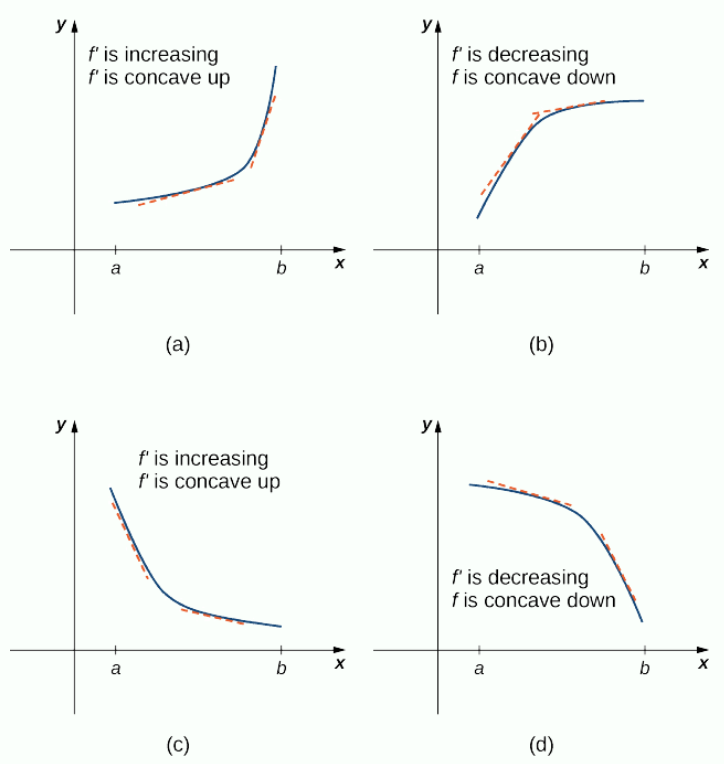
\includegraphics[scale=0.6]{img/image-20200413135215226.png}
\end{fullwidth}

A point \(P\) on a curve \(y=f(x)\) is called an
\textbf{\emph{inflection point}} if \(f\) is continuous at \(P\) and the
curve changes the direction of concavity at \(P\).

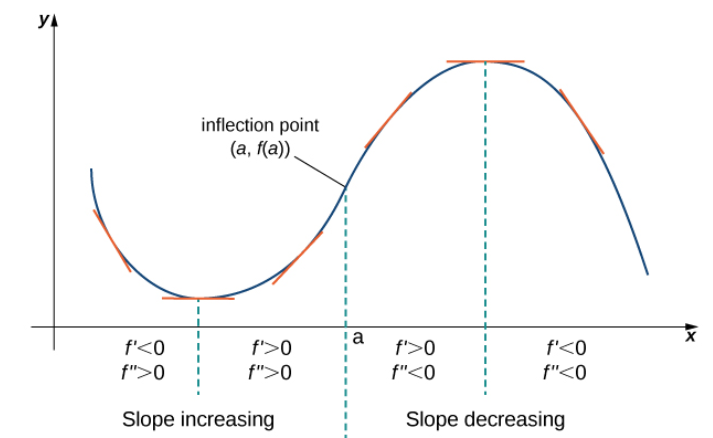
\includegraphics[scale=0.4]{img/image-20200413135252785.png}

\end{definition}

\begin{proposition}

\textbf{(Concavity Test)} Let \(f\) be a function on \((a, b)\).

\begin{enumerate}[sepno]
\item
  If \(f''(x)>0\) on \((a, b)\), then \(f\) is concave upward on
  \((a, b)\).
\item
  If \(f''(x)<0\) on \((a, b)\), then \(f\) is concave downward on
  \((a, b)\).
\end{enumerate}

\end{proposition}

\begin{example}

For the function \(f(x)=x^3 - 6x^2+9x+30\), determine all intervals where
\(f\) is concave up and all intervals where \(f\) is concave down. List
all inflection points for \(f\).

\end{example}
\vspace*{6\baselineskip}

\begin{proposition}

\textbf{(Second Derivative Test)} Let \(f\) be a function defined on
\((a, b)\). Assume that there is a number \(c\) in \((a, b)\) such that
\(f'(c)=0\) and \(f''(c)\) exists.

\begin{enumerate}[sepno]
\item
  If \(f''(c)<0\), then \(f\) has local maximum value at \(c\).
\item
  If \(f''(c)>0\), then \(f\) has local minimum value at \(c\).
\end{enumerate}

\end{proposition}

\begin{example}

Consider the function \(f(x)=x^3 - \frac{3x^2}{2} - 18x\). Use the second
derivative test to determine local extrema of \(f\).

\end{example}
\vspace*{6\baselineskip}

\begin{example}

Let \(f(x)=x^3-6x^2\).

\begin{enumerate}
\item
  Find the intervals where \(f\) is increasing and where it is
  decreasing.
\item
  Find the local extrema if they exists.
\item
  Find the interval where \(f\) is concave upward and where it is
  concave downward.
\item
  Find the inflection points if they exits.
\end{enumerate}

\end{example}

\subsection{Practice}

\begin{exercise}

Determine intervals where \(f(x)=\sin x+\sin^3x\), where \(0<x<\pi\), is
increasing or decreasing.

\end{exercise}
\vspace*{6\baselineskip}

\begin{exercise}

Use the first derivative test to find the location of all local extrema
for \(f(x)=x+x^2 - x^3\).

\end{exercise}
\vspace*{6\baselineskip}

\begin{exercise}

For the function \(f(x)=x+\sin(2x)\) over
\([\frac{\pi}{2},\frac{\pi}{2}]\),

\begin{enumerate}
\item
  determine all intervals where \(f\) is concave up or concave down;
\item
  list all inflection points for \(f\).
\end{enumerate}

\end{exercise}

\begin{exercise}

Consider the function \(f(x)=\sin(\pi x)-\cos(\pi x)\) over
\(x=[-1,1]\). Determine

\begin{enumerate}
\item
  intervals where \(f\) is increasing or decreasing,
\item
  local minima and maxima of \(f\),
\item
  intervals where \(f\) is concave up and concave down, and
\item
  the inflection points of \(f\).
\end{enumerate}

\end{exercise}

\begin{exercise}

Consider the function \(f(x)=\frac{1}{1 - x}\), where \(x\neq 1\).
Determine

\begin{enumerate}
\item
  intervals where \(f\) is increasing or decreasing,
\item
  local minima and maxima of \(f\),
\item
  intervals where \(f\) is concave up and concave down, and
\item
  the inflection points of \(f\).
\end{enumerate}

\end{exercise}

